\subsection{Product perspective} 
The product we will develope is a software application  for smartphone implementing Android as operative system. The app will require the user to be registered in order to access to all the funtionalities. It will also need a stable internet connection in order to connect to different external system providing information about weather and transport means. The application runs locally on the smartphone but users data are also stored in the the system database.

\begin{figure}[!h]
	\centering
	\makebox[\textwidth][c]{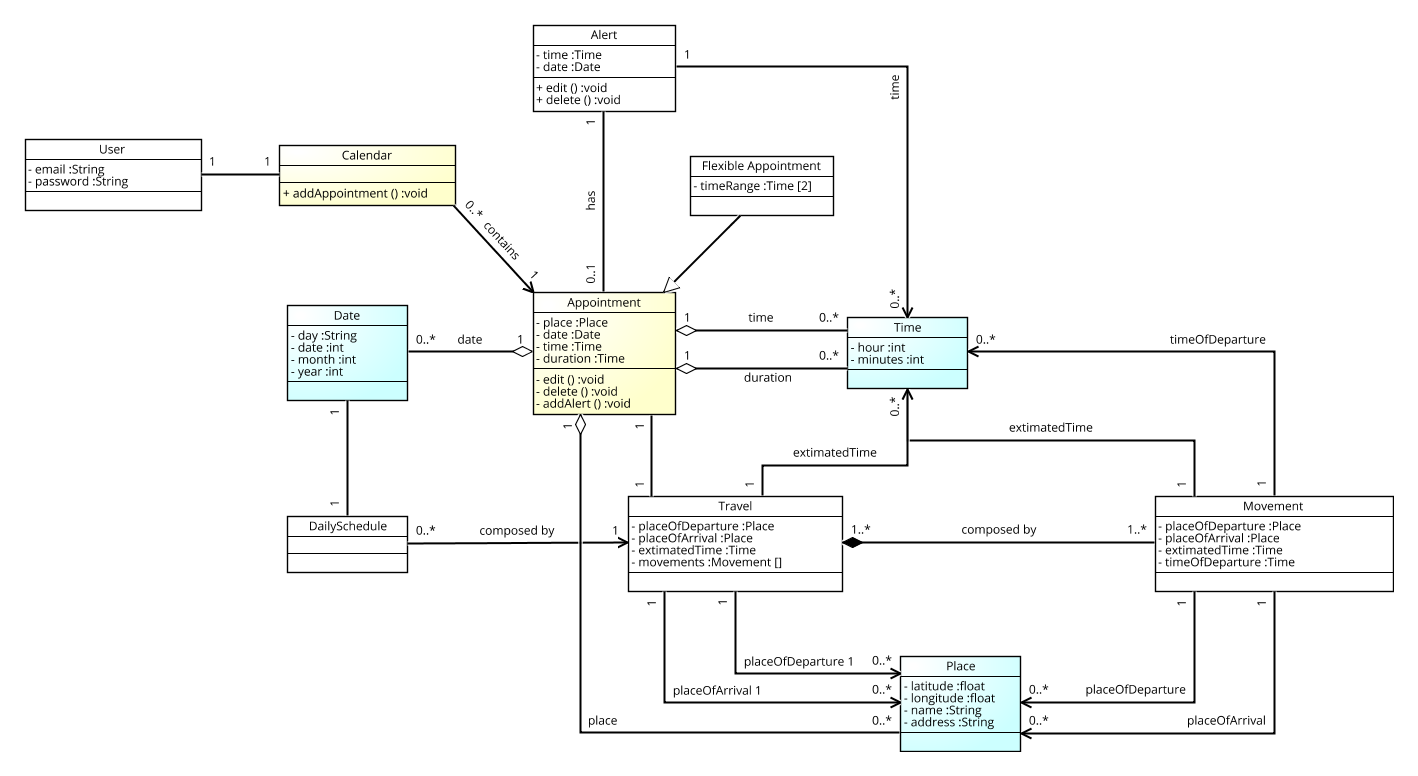
\includegraphics[width=1.2\textwidth]{Images/ClassDiagram.png}}%
\end{figure}

(UML e stateCharts)

\subsection{Product functions}
This application aims to provide a smart and user-friendly appointment-manager system, which allows the user to create and keep track of several appointment on a personal virtual calendar. Plus, the app is able to schedule the travels to reach the different appointment destinations on time in the fastest and most confortable way, according to the preferences expressed by the user and the different weather and public transport condition. Finally, the application offers the possibility of easily buy tickets for the different trips, and to view them when needed.
\subsection{User characteristics}
We recommend the application to a person who wants to organize easily his time in the best way. He will be able to benefit from this service in a very simple way because Travlendar+ requires only basic knowledge of a simple calendar. After registering an account, the application is ready to handle his commitments, so scheduling the best organization.
\subsection{Domain Assumption and Dependencies}
\begin{itemize}
	\item For any day user can create unlimited number of events.
	\item User has only one calendar.
	\item There isn’t any dependence between users.
	\item User can choose among some alternative travel proposals.
	\item If an event is overlapping another one, the user must select a choice from the choices proposed.
	\item User can delete an event.
	\item User can modify an event already created.
	\item User can change the scheduling proposed.
	\item User can select in which preferences the scheduling based on.
	\item Notification of best proposal will be shown.
	\item Notification of any problem that occurs will be shown.
\end{itemize}
\subsection{Constrains}
Travlender+ requires:
\begin{itemize}
	\item Internet connection enabled on own device
	\item GPS available on own device
	\item Login during the first access
	\item Initially registration with an account
	\item Android device
	\item Milano as the default city
	\item 30 Mb(?) of storage memory available on own devise to be installed
\end{itemize}


